\subsubsection{Job Queue Page Specifications}
The Job Queue page helps the user see the status of jobs started using the Job Creation page. A job has five possible statuses, including finished, failed, cancelled, queued, and processing. These, along with the functionality of the Job Queue, are shown in the image below.\\
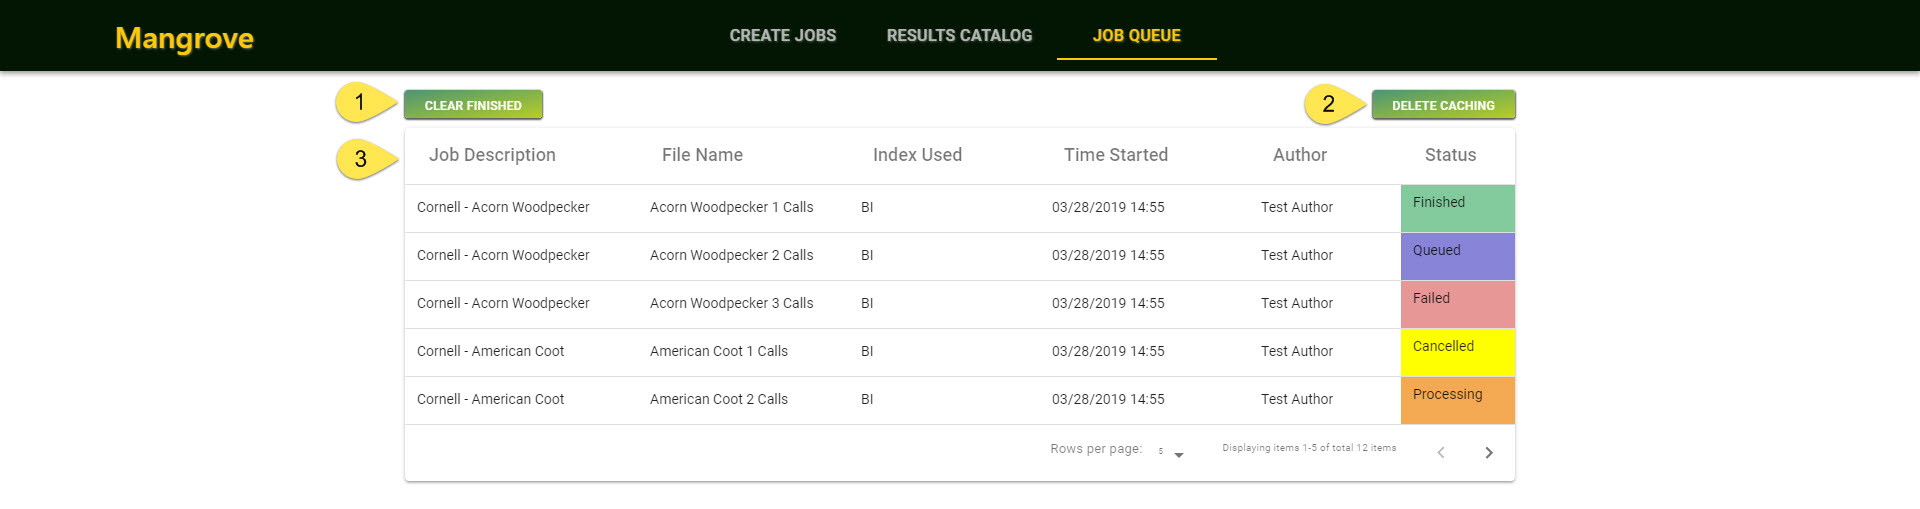
\includegraphics[width=\textwidth]{jobQueue}
\begin{enumerate}
  \item \textbf{Clear Finished}\\ This button allows the user to remove any jobs with the finished status. This helps clean up the job queue and show only those jobs that are waiting to be processed, or are in the process of doing so, or those that failed.
  \item \textbf{Delete Caching}\\ This button will remove all jobs in the job queue regardless of status. This button is more to be used as an error handler, if some error occurs during processing.
  \item \textbf{Job Queue}\\ The actual queue itself is organized as a table containg a job description of the site and series, author, and the file name itself. Additionally, the index being used in the job and the time started are available. Finally, the job status is color coded in the last cell.
\end{enumerate}
